\documentclass{article}
%graphique
\usepackage{epsfig,graphicx,float}
%math
\usepackage{amsmath}

\newcommand{\be}{\begin{equation}}
\newcommand{\ee}{\end{equation}}
\usepackage{graphicx}

%----------NE PAS MODIFIER CE QUI EST AU DESSUS-------------

\begin{document}


\author{ JG Caputo}
\title{Simulation de l'\'evolution d'une population dans le temps}

\date{\today}
\maketitle


\section{Le projet}
Le but du projet est de realiser un programme en C permettant le calcul de l'evolution d'une population durant n mois :
$$x_{n+1}=f(x_n)$$ o\`u $$f(x)=a(x_n( 1 - x_n )$$ si$$x\leq{4}$$
L'equation est ecrite sur une ligne a part avec les \$\$. Si on met un
seul \$ la formule est inseree dans le texte.
On peut aussi utiliser begin/ end \{equation\} (alias be,ee)
Ca donne
\begin{equation}  \label{eq1}
x_{n+1}=f(x_n) . \end{equation}
Si il y a plus d'une equation, on utilise l'environnement eqnarray
\begin{eqnarray}  
x_{n+1}= a x_n + b y_n , \label{eq2}\\
y_{n+1}= c x_n + d y_n , \label{eq3}.
 \end{eqnarray}
Pour les references on utilise cite, par exemple \cite{crs01}. Les references
sont mises avec des bibitem a la fin du fichier.


\section{Mise en oeuvre informatique}

Code permettant d'obtenir les diagrammes d'evolution de la suite en fonction de n, suivant les valeurs de a.

\begin{verbatim}

#include<stdlib.h>
#include<stdio.h>
#include<math.h>



int main()
{
int jk, k;
float a, p0, p1, var;
		scanf("%d %f %f",&jk, &p0, &a);
	for( k = 1 ; k <= jk ; k++)
	{
		p1 = a*p0*( 1 - p0 );
		var = ( ( p1 - p0) / p0 )*100;
		printf("%d  %f %f \n",k, p1, var );
		p0 = p1;

	}
}


\end{verbatim}


Code permettant d'obtenir le diagramme de bifurcation, c'est a dire celui donnant les valeurs des points des points fixes en fonction de a.



\section{Etude Mathematique}

     Expression initiale : $$x_(n+1) = ax_n(1 - x_n)$$ pour  $$0 < a < 4$$
  c'est a dire $$x_(n+1) = f(x_n) = ax_n(1 - x_n)$$

On peut inserer les fichiers graphiques postcript (.eps ou .ps) avec
epsfig voir Fig. \ref{fig1}. Les autres formats graphiques .jpg .png
peuvent etre inseres avec includegraphics  voir Fig. \ref{fig2}.

%Insertion d'une figure en eps dans le texte avec epsfig
\begin{figure} [H] \label{fig1}
\centerline{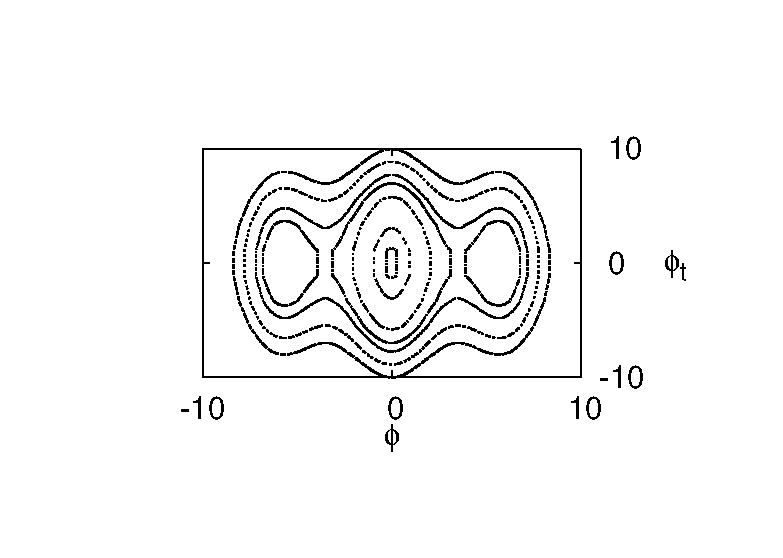
\epsfig{file=ham.eps,height=6cm,width=12 cm}}
\caption{Facon avec epsfig}
\end{figure}

\begin{figure} [H]
\centering
\resizebox{14 cm}{5 cm}{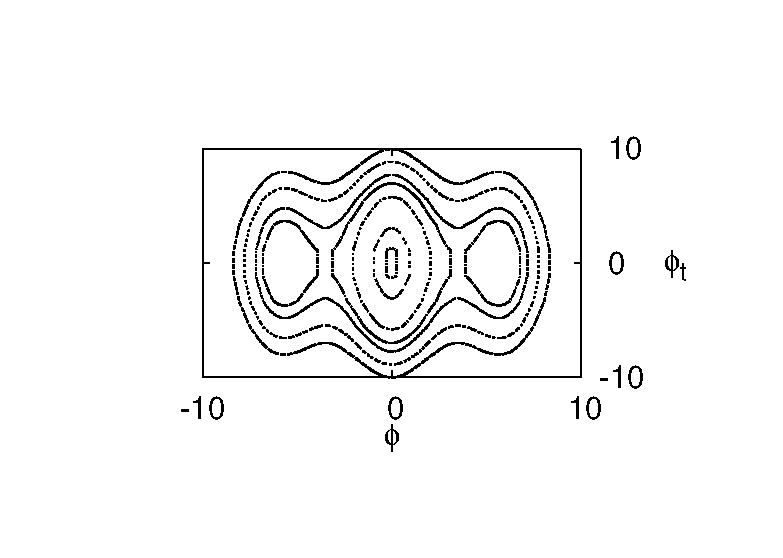
\includegraphics{ham}}
  \caption{Une facon avec includegraphics}
  \label{fig2}
\end{figure}



 Recherche des points fixes :

  On pose x* un point fixe, c'est a dire $$x* = f(x*)$$
  Resolution de l'equation : $$x* = ax*(1 - x*) $$
  D'ou $$x* = 0$$ et $$x* = (a - 1)/a$$


\begin{thebibliography}{99}


\bibitem{crs01} D. Cvetkovic, P. Rowlinson and S. Simic,
 "An Introduction to the Theory of
Graph Spectra",  London Mathematical Society Student Texts (No. 75), (2001).
\end{thebibliography}


\end{document}
